\chapter{Building Accessible and Automated Mass Cytometry Analysis Tools}
\label{03cytof}

\section{Introduction}


As outlined in the background section, the mass cytometry platform used to analyse the CRC organoids is already a mature approach. With a previously characterised model, the effects of both TME and genotypical perturbations have also been described, but the data analysis was done using custom and discrete scripts; encumbering consistency and reproducibility for future analyses. Manual gating too for cell state.

% cygnasl
To improve upon this I have designed and developed CyGNAL (CyTOF SiGNalling AnaLysis)20, a pipeline for mass cytometry data analysis with a focus on studying PTM changes across multiple conditions. 
\colorbox{yellow}{Under continued development and in revision at Nature Protocols, CyGNAL aims to streamline and bring to non-computational scientists analyses similar to those shown in Qin et al. 202011, with the addition of dimensionality reduction embeddings and interactive visualisations.}
Applied to analsie datasets, works in conjucntion with tobis mc and multiplexed cytof panels on organoids as shown in Sufi \& Qin et al. \cite{sufi_multiplexed_2021}.

%class
The maturity of the platform is also reflected on the properties of the markers used in the mass cytometry panels, with the most robust markers achieving highly binary and specific staining. Given the importance of cell state changes to perturbations in the epithelial organoids, either in the form of intrinsic effects such as genotype or extrinsic in the form of the TME or drug treatments, an automated approach of labelling and assigning a cell state to each cell in an experiment would facilitate routine analysis of mass cytometry datasets. 
I thus hypothesise that we can use a machine learning approach to, using a series of canonical cell state markers, automatically predict and label the hundreds of thousands of cells captured in a mass cytometry experiment. To this end I aim to develop a random-forest classifier. This classifier will be able to ingest mass cytometry datasets and, using manually gated datasets with cell state labels as training data, label each of the cells with one of six possible cell states: Apoptosis, G0, G1, S-phase, G2, and M-phase. 

\section{CyGNAL: CyTOF Signalling Analysis pipeline}

Published and demoed as part of Sufi \& Qin et al. 2021, CyGNAL is a publicly available tool that is routinely used to analyse mass cytometry datasets both at my group and by external collaborators \cite{michelozzi_activation_2023}.

Details on the implementation, code structure and deployment can be found in Chapter \ref{02methods}. Furthermore, a step-by-step walk-through of the main CyGNAL steps is detailed in Sufi \& Qin et al. \cite{sufi_multiplexed_2021}.

In this section I will present an overview of the tool and will discuss the relevance of the different scoring systems with regards to mass cytometry data in general and PTM signalling panels in specific. Example outputs from CyGNAL will also be shown, both for it's non-interactive sections (scores and UMAP embedding) and how they can be further analysed, but also with screenshots of the interactive apps that constitute CyGNALs visualisation steps.

\subsection{Overview and Capabilities}
% \subsection{}{Pipeline modules}

CyGNAL is a collection of scripts written mainly in Python and R. These scripts have been built around a unified code base of shared functions and a particular directory structure to facilitate interoperability between the different steps. 

Within CyGNAL's code directory, the utils folder has optional steps that either complement the main ones or belong to additional utilities for handling mass cytometry datasets. 

Distribution of CyGNAL is accomplished as a container hosted in Docker Hub (\href{https://hub.docker.com/repository/docker/ferranc96/cygnal}{hub.docker.com/repository/docker/ferranc96/cygnal}). CyGNAL can also be used by downloading the project's public repository (from \href{github.com/TAPE-Lab/CyGNAL}{github.com/TAPE-Lab/CyGNAL}) and then installing all required Python and R dependencies via conda using the provided YML environment file. More details on this process can be found in Chapter \ref{02methods}.

The tool relies on the computation of two scores, EMD and DREMI, to analyse the intensity of detected antibodies across conditions or other gating-derived metadata groups (i.e. cell-cycle phase or cell type). EMD describes the distance between distributions of detected intensities, and thus is used to compare protein expression across conditions. DREMI is a mutual information estimate that can be used to relate the degree of connectivity across conditions of protein pairs. More details on both methods and how they are implemented can be found in Chapter \ref{02methods}.

\begin{figure}
    \centering
    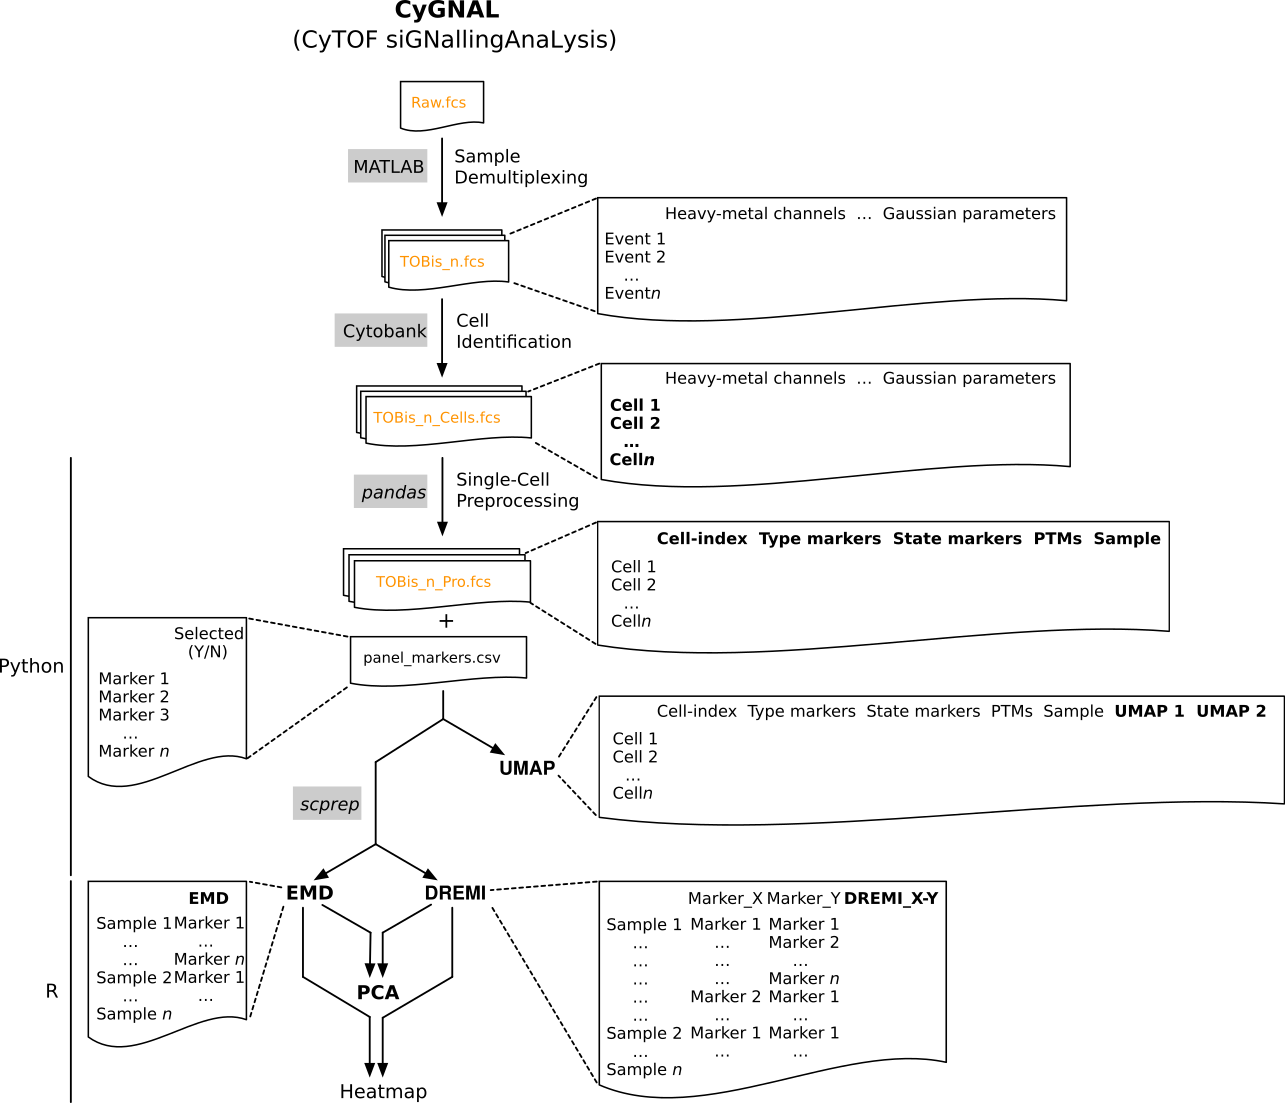
\includegraphics{03cytof/figs/3CYGNAL_pipeline.png}
    \caption{PIPELINE CYGNAL. WIP, consider merging with the use case figure as the overlap is significant.}
    \label{fig:3cygpipe}
\end{figure}

A general overview of CyGNAL's structure is shown in Figure \ref{fig:3cygpipe}, where the tool encompasses the bottom two thirds of the diagram.

As CyGNAL uses FCS files or tab-separated plain text files, certain upstream processes are necessary after data acquisition. Previous to analysing the data in CyGNAL, the standard operating procedure in our lab is to debarcode the mass cytometry datasets in MATLAB (using the tool from \href{github.com/zunderlab/single-cell-debarcoder}{github.com/zunderlab/single-cell-debarcoder}) and perform initial data pre-processing and quality control in Cytobank (\href{www.cytobank.org}{www.cytobank.org}). In that platform, the single cells are gated for Gaussian parameters, their DNA content, and uptake of Cisplatin using manual gates. Gating on cell state and cell type specific markers can also be done in order to both eliminate doublets but also to identify cells belonging to each state or type; information which can then be used to train the cell state classifier among others.

CyGNAL proper starts with the pre-processing step. Here, empty heavy metal channels with no conjugated antibodies are removed, and the remaining channels are renamed to reduce the presence of special characters and keep with the naming conventions of the Fluidigm CyTOF software. A unique cell identifier is also given to each cell, and experiment metadata can also be embedded within the main pandas dataframe. Furthermore, a file with update antibody channel names is also saved (panel\_markers.csv), so that the user can select which channels to use in downstream steps.

Dimensionality reduction via Uniform Manifold Approximation and Projection (UMAP)\cite{mcinnes_umap_2020} can be performed to embed the individual cells on a 2-dimensional space based on the select antibodies.

EMD and DREMI scores are computed using the scprep package \cite{noauthor_krishnaswamylabscprep_2021}. Compute time can be reduced by subsetting the panel to channels of interest, and the user gets prompted to define specific arguments relevant to either computation, such as defining the variable and reference distributions for the EMD step.

Finally, the computed EMD and DREMI scores can be visualised as heatmaps or further summarised via PCA to compare profiles across conditions using CyGNALs last two main steps. The visualisation steps load in the default and user-given parameters and pass them to R Shiny-Apps \cite{noauthor_rstudioshiny_2021} that host a local server which automatically opens on the browser.

\subsection{Use Case and Outputs}

CyGNAL is distributed with sample mass cytometry datasets, which originate from technical replicates of an organoid monoculture experiment. They have been downsampled so that they can be hosted on GitHub and distributed with the code itself. The results presented in Figure \ref{fig:3cygvis} A-C were generated with this sample data.

In Figure \ref{fig:3cyguse} I present a mass cytometry dataset from Qin et al. 2020 \cite{qin_cell-type-specific_2020} to showcase an example use with heterotypic culture conditions where cell type specific analysis is necessary. The data belongs to the same mouse colon organoid model from Chapter \ref{04seq} and presents with a similar experimental setup, wherein organoids with different genotypes where cultured on their own or with macrophages and/or fibroblast cells. Data was subsequently gated and annotated on cell types and states as described above and on the original publication \cite{qin_cell-type-specific_2020}, and then passed onto CyGNAL for preprocessing (Figure \ref{fig:3cyguse} A).

\begin{figure}
    \centering
    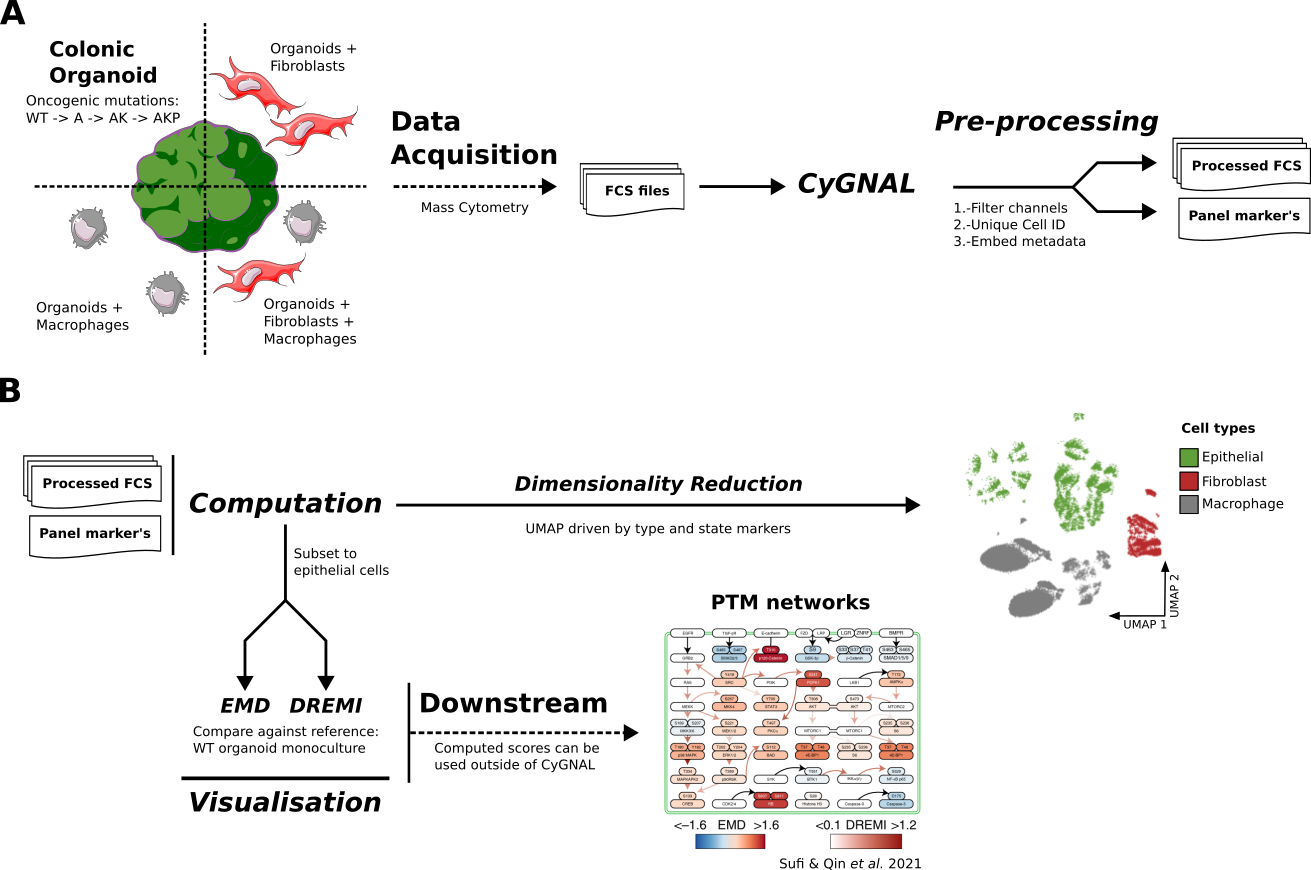
\includegraphics{03cytof/figs/3CYGNAL_usage.png}
    \caption{}
    \label{fig:3cyguse}
\end{figure}

Panel markers files use to select state and type markers to be used for umap computation. pHH3, IdU, cCasp3, pRB, LRIG1, CEACAM1, pan-CK, F4/80, PDPN, RFP, CyclinB1, CD68. Embedding resolves the three distinct types (Figure \ref{fig:3cyguse} B).

Using the cell-type gates previously drawn on Cytobank, unique cell identifiers were used to select only the organoid cells. Computation of EMD and DREMI scores was then performed on the epithelial compartment, and can be visualised as part of CyGNAl. Furthermore, in the specific context of PTM network signalling analysis, EMD and DREMI scores can be used to assemble signalling network diagrams. With EMD used to quantify PTM node intensity and DREMI to score PTM-PTM edge connectivity, a signalling network can be curated and manually annotated as shown in Qin et al. 2020 \cite{qin_cell-type-specific_2020}. 

When paired with a well-curated antibody panel and robust experimental design, TOBis MC allows multiplexed analysis of cell type–specific PTM signalling of heterocellular organoids \cite{sufi_multiplexed_2021}. 

\begin{figure}
    \centering
    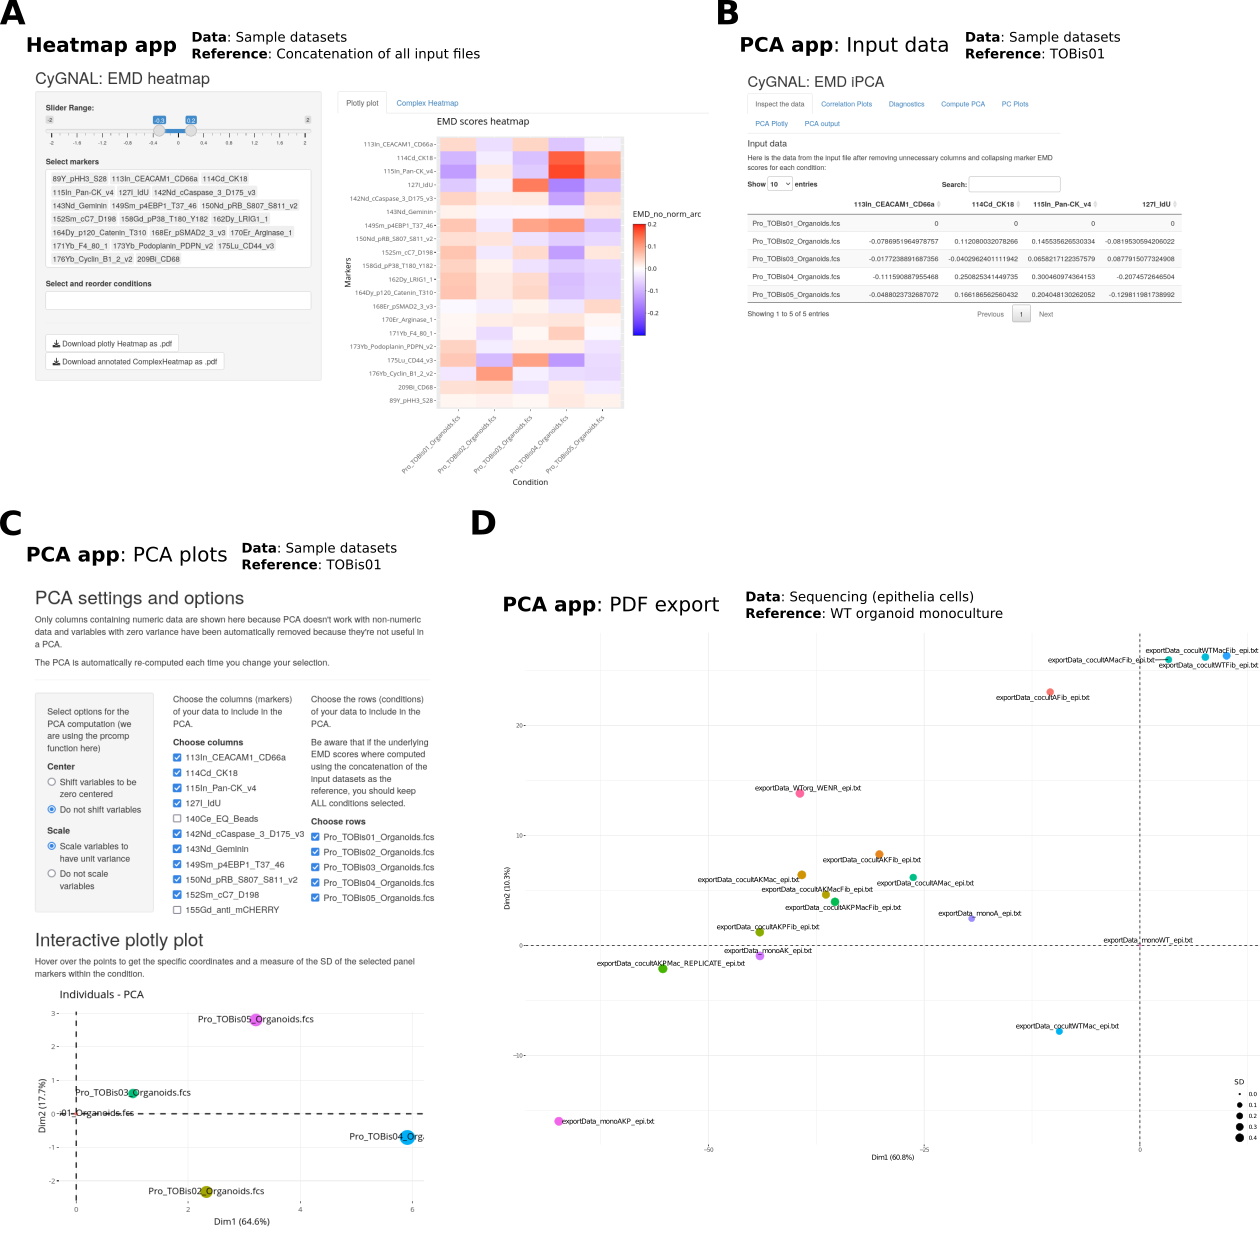
\includegraphics{03cytof/figs/3CYGNAL_usageVIS.png}
    \caption{}
    \label{fig:3cygvis}
\end{figure}

Using the sample data and with the concatenation of all input files as the reference for the EMD step, Figure \ref{fig:3cygvis}A demonstrates CyGNAL's heatmap visualisation. By selecting not to use a specific reference during the EMD computation step, the generated scores are useful to compare how antibody expression compares across each of the individual datasets/conditions. The heatmap ShinyApp lets the user control the colour scale (automatically set to maximise contrast on the range of EMD scores), remove antibodies from the heatmap, and reorder the datasets/conditions shown in the columns. The heatmap shown in Figure \ref{fig:3cygvis}A is an interactive version generated with Plotly \cite{plotly_technologies_inc_collaborative_2015}, and shows the corresponding EMD score when hovering over a cell. Furthermore, a similar non-interactive heatmap is generated using the ComplexHeatmap \cite{gu_complexheatmap_2021} package and can be found within its homonymous Shiny-App tab.

The same data was used when running the PCA Shiny-App in Figure \ref{fig:3cygvis}B-C. This CyGNAL steps lets the user explore the data by looking at the raw scores (Figure \ref{fig:3cygvis}B) and Pearson correlation between channels. The user can also define parameters for the Principal Components Analysis, including the number of markers, generate several types of PCA plots with or without eigenvectors overlaid, and export the PCA results as plain text. In Figure \ref{fig:3cygvis}D I demonstrate how, despite CyGNAL being originally designed to handle mass cytometry data, other types of singl-cell omic data like scRNA-seq can also be used. Here I used CyGNAl to compute EMD scores based on the gene expression of the organoids sequenced in Chapter \ref{04seq} and generate a PCA embedding showing how the different conditions compared to the control.
Note that the PCA data in Figure \ref{fig:3cygvis}B-D was generated using EMD scores computed with a particular dataset/condition as the reference and without centring the PCA embedding matrix, exemplifying use cases where we have a clear control condition against with the other conditions are compared (like the WT organoid monoculture in Figure \ref{fig:3cygvis}D).


\section{Cell-state Random Forest Classifier}

General idea of gating done on limited subset of markers is what determines cell state. Process naturally resembles decision trees (threshold of antibody intensity results in binary output). Random forest as an ensemble approach that can automate the gating process.

\begin{figure}
    \centering
    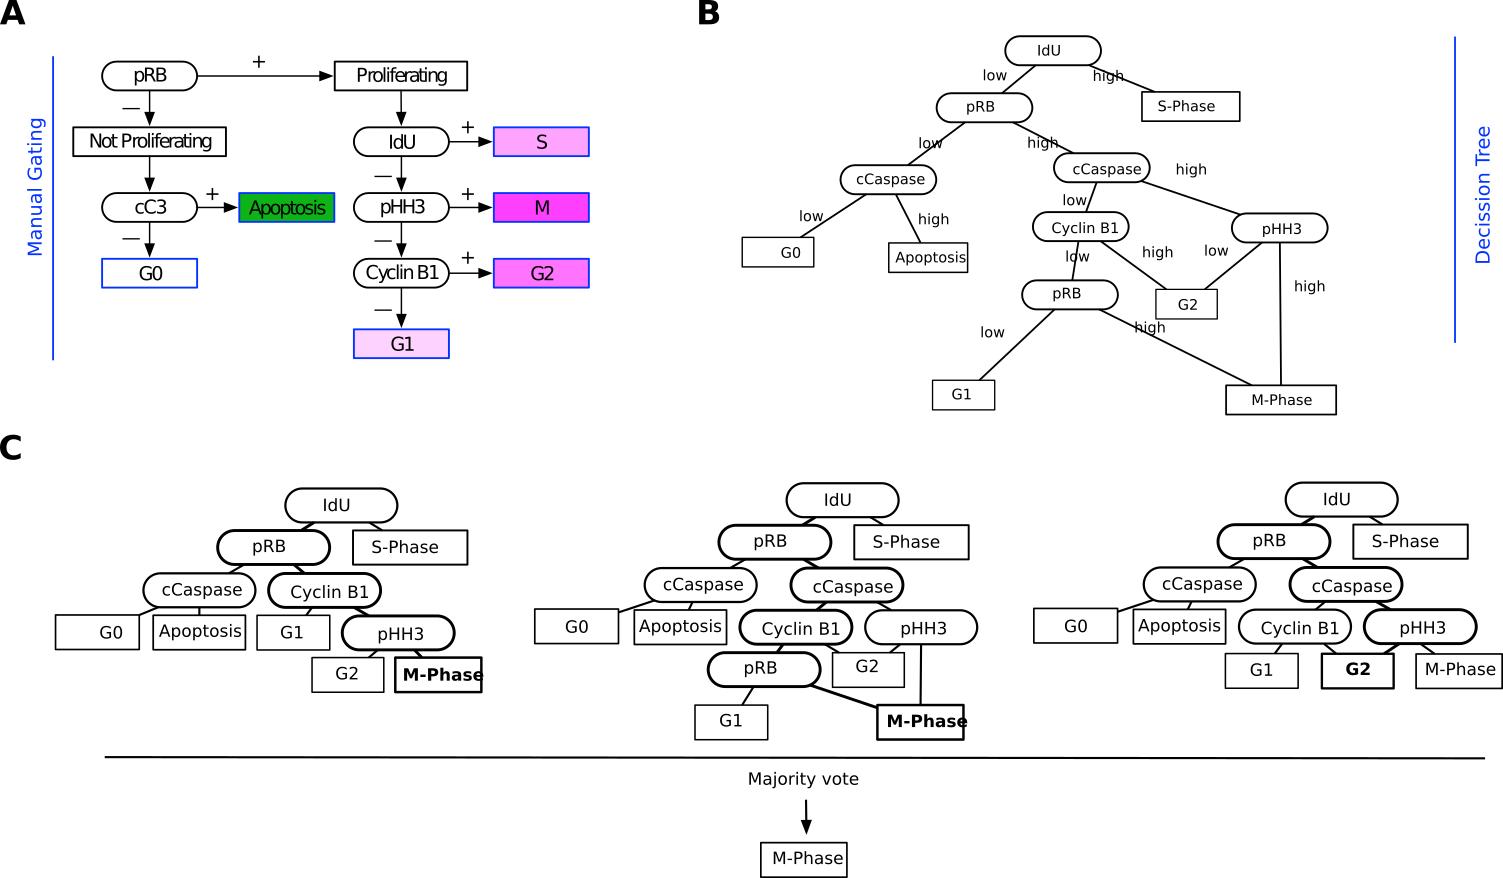
\includegraphics{03cytof/figs/3CLASS_stateRF.png}
    \caption{}
    \label{fig:3classover}
\end{figure}

\subsection{5-marker model:baseline}

Testing the 5-marker RF model on a single time-point SI LGR5 organoid culture11 results in global accuracy for all classes of 0.93. However, looking at the classification report in Figure 3 a) we see how there is a significant drop of f1-scores when classifying the apoptotic class, scores which otherwise remain above 0.92. This fall in f1-scores seems to be driven by a low precision (0.5) when classifying cells as apoptotic.
Performance of the classifier drops when testing against the CRC TME colonic organoid cultures from Qin et al. 2020. In this case, when we subset just the organoid cells from the organoid cultures (i.e., by extracting all epithelial cells irrespective of the genotype or the other cell types they might have been analysed with), we observe a global accuracy of 0.91. Looking at the classification details (Figure 3 b.) we see a very similar pattern to the SI LGR5 results; with the apoptotic class presenting the lowest f1-scores (0.6) characterised by a low precision (0.43). Furthermore, the remaining f1-scores are also lower overall, with only the S-phase and M-phase classes reaching above the 0.9 mark.

When instead of subsetting just the organoid cells we test against all cells from the CRC TME dataset (i.e., including also fibroblasts and macrophages) global accuracy drops down to 0.87. The relatively high global accuracy does not reflect the failure of the classifier to, yet again, identify the apoptotic cells (see Figure 3 c.). In Figure 3 d) the classification matrix is used to build a dot plot in which the true labels (“Real state” from gating) are compared against the predicted labels (“Predicted state”), highlighting how a majority of the cells labelled as apoptotic are actually G0 cells, explaining the precision of 0.32 for the former class. There is also some confusion around the G2 cells, as a significant number of these cells are classified as either G0 or G1.

\begin{figure}
    \centering
    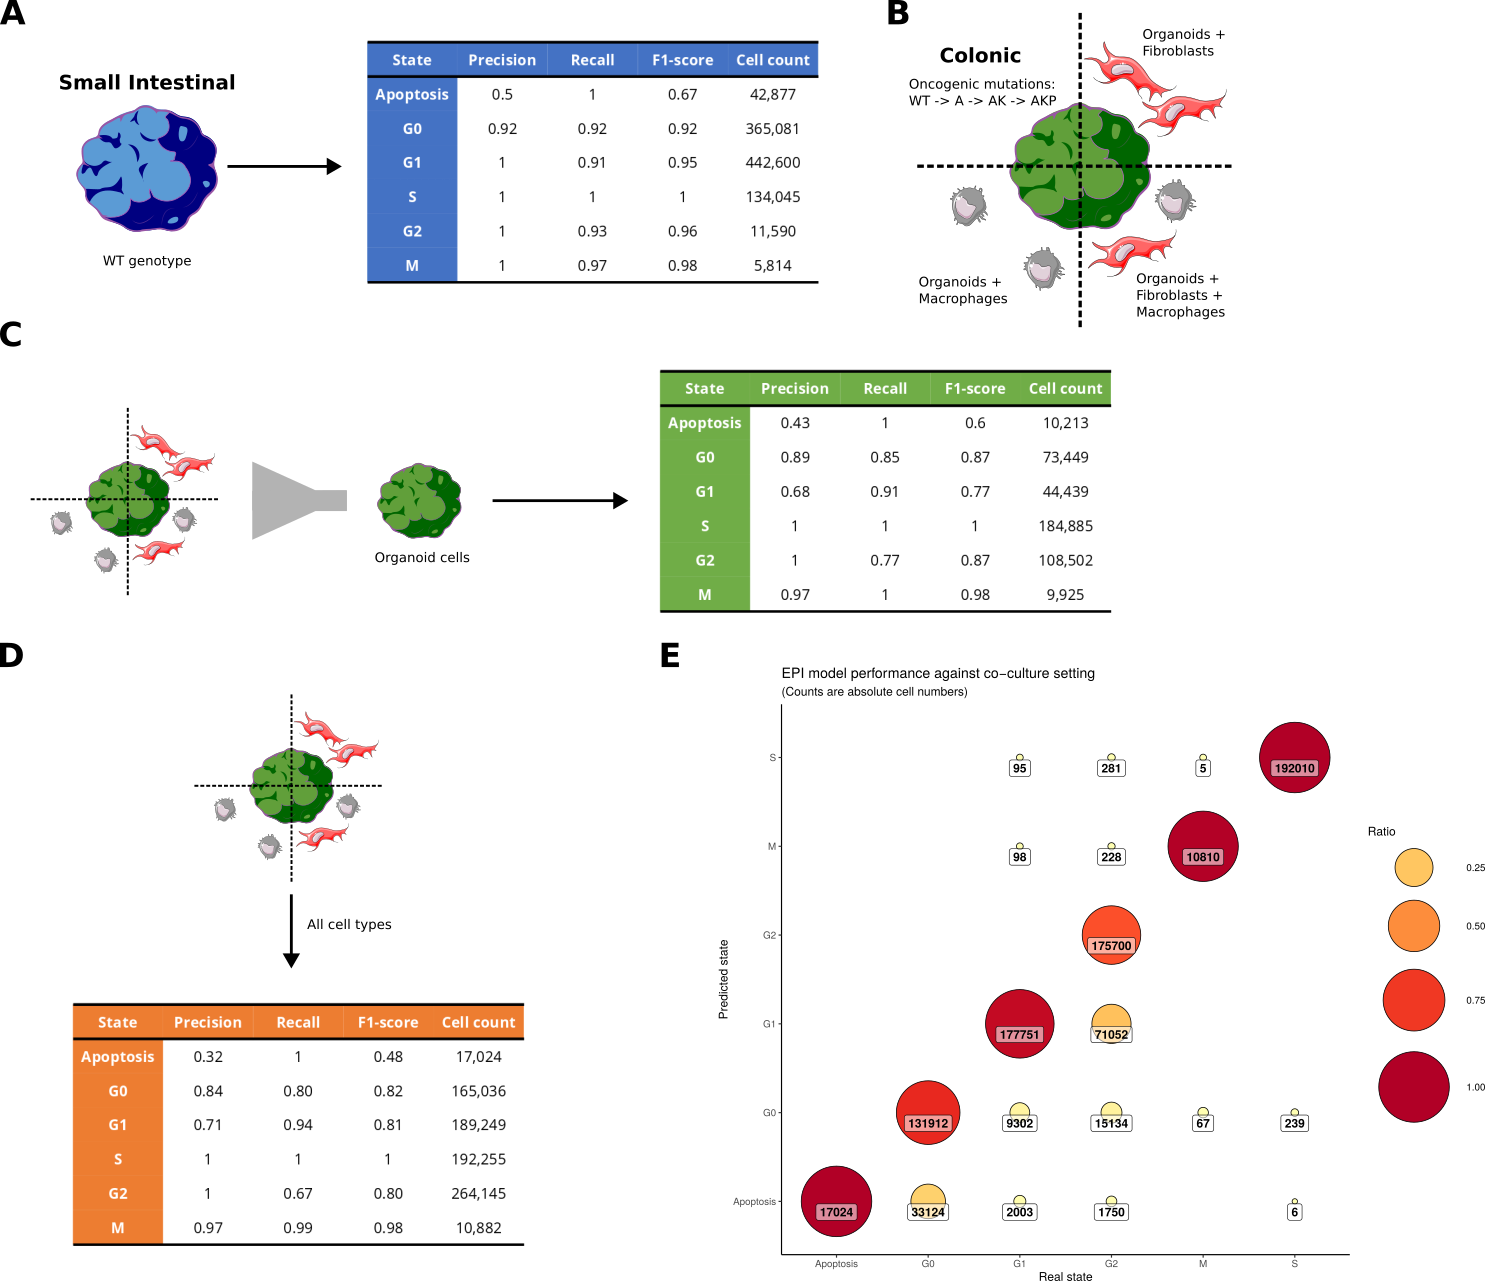
\includegraphics{03cytof/figs/3CLASS_5m.png}
    \caption{}
    \label{fig:3class5m}
\end{figure}
 
Figure 3: Benchmarking 5-marker RF cell state classifier. Shown in a), b), and c) are the classification reports obtained from running the 5-marker RF classifier against data manually labelled for cell state (representing the “real state” or ground truth). In a) a single timepoint SI LGR5 dataset was used, very similar to the training data for the model. The dataset in both b) and c) is a coculture of CRC organoids and their TME, with the cells in b) being a subset of the whole dataset containing just epithelial cells. Decreasing levels of performance correlate with increasing differences between the train and test datasets, as can be seen by the low f1-scores for the apoptotic class in c). Using the same data as c), the dot plot derived from the classification matrix in d) depicts the number and proportion (as both size and colour of the circles) of mislabelled cells for each cell state, showing that a considerable number of falsely mislabelled apoptotic cells are actually in G0 phase and some cells. RF: Random Forest.



\subsection{10-marker model improves apoptotic classification}

Cross species, on PDO chemotherapy data. data from \cite{zapatero_trellis_2023}.

Preliminary benchmark results from the updated 10-marker implementation using PDO data show improved performance when compared to the 5-marker model. In this case we observe a global accuracy greater than 0.99, with the lowest f1-score being of 0.95 for the cells in M-phase (see Figure 4 a.). In the classification matrix in Figure 4 b) we observe how, given the lower total count of M-phase cells (true label = 5, one order of magnitude smaller than the other classes), small numbers of misclassified cells (mainly as G2 and S-phase predicted labels, represented by the numbers 4 and 3 respectively) drive down the recall for the M-phase class. 
In contrast with the 5-marker model results, there is an apparent lack of issues when classifying the apoptotic class, with only 0.35% of true apoptotic cells being mislabelled. A bar plot representing the importance of each feature during classification is shown in Sup. Figure 2.

Above is tested with a dataset containing both a technical replicate fro m the training data and a different dataset where organoids have when treated with the chemotherapy SN38 \colorbox{yellow}{check right name and conentration}. 

\begin{figure}
    \centering
    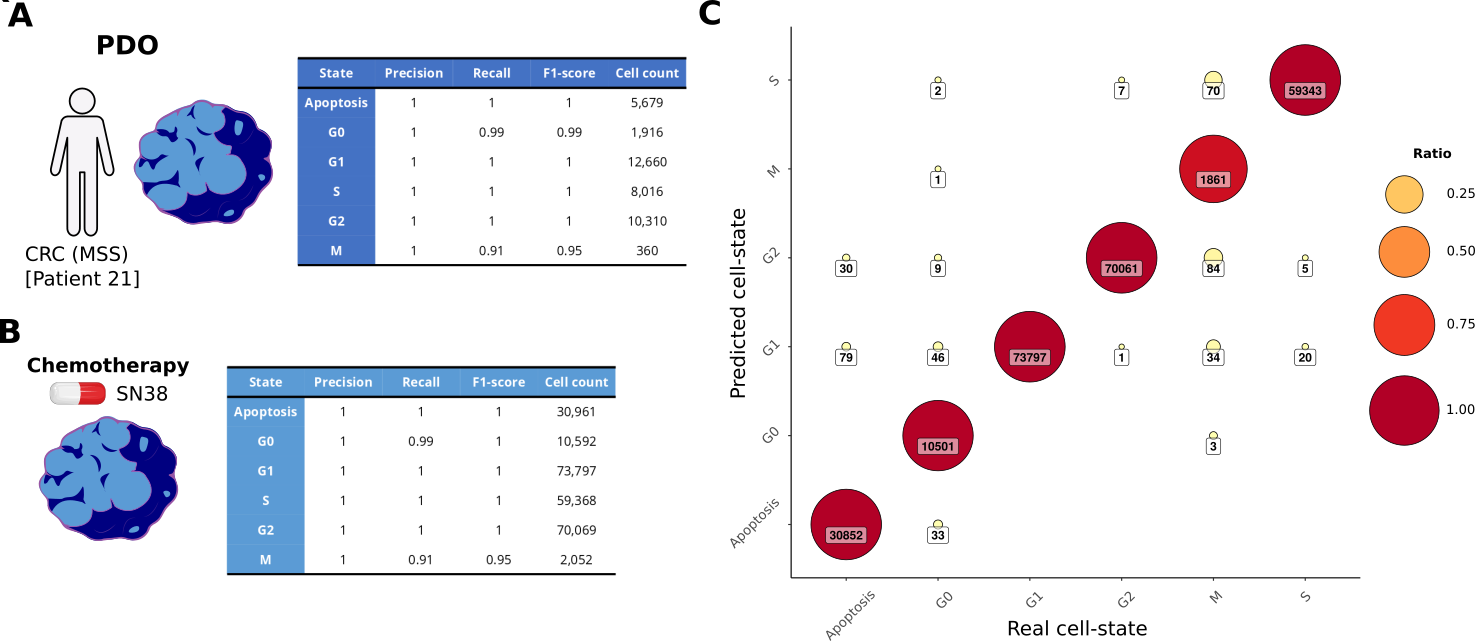
\includegraphics{03cytof/figs/3CLASS_10m.png}
    \caption{}
    \label{fig:3class10m}
\end{figure}
 
Figure 4: Benchmarking the new 10-marker RF cell state classifier. Building a RF classifier with an increased number of markers using data from PDOs renders better results than the original 5-marker model, as can be seen in a) with the classification report. b) Classification matrix generated automatically during model building, showing extremely low levels of misclassified cells. RF: Random Forest. PDO: Patient-Derived Organoids. Labels: 0=Apoptosis, 1=G0, 2=G1, 3=S-phase, 4=G2, 5=M-phase.

% \subsection{Tested on externally cytof data}



\section{Conclusions}

cygnal can be used for explor analysis and even publi grade results -> do we have ref to substantiate this statement though?
Utils folder and continuous growth. Feedback from users int he lab paramount when defining these utilities.

classifier simple model that works due to limited number of markers and gating nature of current manual state classes. Robust and generalisable expected weak points.
This classifier shows link PTM->cellSTate, also shown in literature and pubs from our lab
Usefullness in determining antibodies not working properly?